\section{Il testing}


Come avviene per qualsiasi oggetto, materiale o immateriale, anche il
processo di sviluppo di un prodotto software può essere suddiviso e schematizzato in una serie di step o fasi. Nella prima fase è necessario individuare e fissare i requisiti che il sistema software dovrà avere, a tale scopo può essere effettuata
un’intervista al cliente da parte del project manager per concordare tali fondamentali caratteristiche; successivamente, il team di sviluppo è incaricato di individuare le tecnologie più efficienti per la realizzazione del sistema ed infine, si passa alla fase di implementazione e collaudo; quest’ultimo, definito in linguaggio
tecnico testing, è il procedimento che viene utilizzato per individuare le differenze tra il comportamento atteso del sistema e quello che invece viene effettivamente
osservato nel sistema software sviluppato.

Tra i vari tipi di testing, è possibile citare i seguenti come esempio:
\begin{itemize}
	\item Testing unitario;
	\item Testing di integrazione;
	\item Testing di accettazione.
\end{itemize}

Essi vengono applicati in successione per effettuare un collaudo del software
a diversi livelli.
\subsection{Testing unitario}
Il testing unitario viene utilizzato per individuare possibili differenze tra le specifiche di un particolare modulo del sistema e la sua realizzazione. In questa fase vengono considerati piccoli \emph{snippet} di codice denominati moduli e vengono testati in maniera indipendente tra loro. Con questa tipologia di testing è possibile
individuare eventuali fault presenti all’interno del modulo stesso.
\subsection{Testing di integrazione}
Dopo aver terminato la fase di testing unitario, lo step successivo prevede l’applicazione del testing di integrazione. In questo caso vengono integrate tra loro tutte le varie componenti create durante la fase di testing unitario e si valuta il comportamento di un determinato modulo nel momento in cui interagisce con un altro.

Esistono diverse strategie per definire l’ordine di integrazione delle varie componenti:
\begin{itemize}
	\item Big Bang: Tutte le componenti vengono integrate contemporaneamente e poi si valuta l’effettiva interazione tra i vari moduli;
	\item Bottom up: Si testano in maniera consequenziale le varie componenti a partire dai layer più bassi fino ad arrivare a quelli più alti;
	\item Top down: Si comincia testando per prime le componenti dei layer superiori, in ordine inverso rispetto a quanto accade nel bottom up;
	\item Sandwich: Combina la strategia del testing Bottom up e quella Top down
	ovvero un team di lavoro inizia a testare le componenti dai layer più bassi a quelli più alti mentre un altro team testa i vari moduli dai layer più alti aquelli più bassi.
\end{itemize}
\subsection{Testing di accettazione}
Il testing di accettazione solitamente implica l’esecuzione di un insieme di casi di test. Ogni caso di test ha lo scopo di sollecitare una particolare funzionalità del sistema.

L’esecuzione di ogni caso di test viene effettuata direttamente nell’ambiente operativo del cliente finale o in alternativa in un ambiente simulato\footnote{Con il termine “ambiente simulato” si intende un ambiente del tutto uguale a quello in cui verrà rilasciato il prodotto software. Tali simulazioni risultano necessarie nel momento in cui si può utilizzare il reale ambiente di lavoro.}. Il test di accettazione può essere eseguito sia dagli sviluppatori del sistema, che dal cliente
finale, prima di mettere in esercizio il sistema sviluppato. Due esempi di testing di accettazione possono essere i seguenti:
\begin{itemize}
	\item Alfa testing: Viene testato il sistema da un numero ristretto di utenti e in un ambiente controllato;
	\item Beta testing: Viene testato il sistema all’interno dell’ambiente in cui sarà messo in esercizio.
\end{itemize}
\section{Metodologia Agile}
La metodologia \emph{Agile} prevede lo sviluppo di piccoli “incrementi” di funzionalità che solitamente sono rilasciati al cliente ogni due o tre settimane denominati \emph{sprint}. Nello sviluppo di prodotti software tramite la metodologia \emph{Agile}
è fondamentale una forte interazione con il cliente, così da ottenere velocemente i feedback necessari alla corretta e pronta soddisfazione di tutte le sue esigenze.
Questa metodologia è stata ideata e sviluppata per l’applicazione a team i cui membri, pur lavorando per lunghi periodi di tempo allo sviluppo dello stesso prodotto software, esercitano la loro attività in aree anche geograficamente distanti tra loro. Gli approcci con metodologie \emph{Agile} vanno a diminuire l’\emph{overhead\footnote{Il termine overhead indica le risorse accessorie che sono richieste per completare un particolare task.}} di sviluppo software, in quanto non prevedono la produzione di gran parte della documentazione che veniva elaborata nel modello a cascata durante la fase di pianificazione, ma si produce documentazione secondo il principio del \emph{“documentare solo quando è necessario”}. Ciò ha permesso ai programmatori di
concentrarsi sullo sviluppo del software piuttosto che sulla fase di progettazione e documentazione dello stesso.
\section{Configuration Management}
I sistemi software sono soggetti a costanti cambiamenti, sia nella fase di
sviluppo che nella fase di rilascio. Spesso essi possono subire cambiamenti sia in risposta a nuovi requisiti, sia in risposta all’introduzione di nuove tecnologie
hardware. Molti sistemi software possono quindi essere considerati come un insieme di versioni differenti, ognuna delle quali dovrà essere mantenuta e gestita
opportunamente.
Il \emph{Configuration Management} (CM) racchiude un insieme di policies, processi e tools necessari per gestire gli eventuali cambiamenti del sistema. Si tratta di uno strumento software che ha le seguenti caratteristiche:
\begin{enumerate}
	\item \emph{Version Control}: Tiene traccia delle molteplici versioni esistenti dello stesso prodotto software sviluppate da diversi programmatori gestendo eventuali conflitti tra le varie versioni;
	\item \emph{System building}: Viene definito come avviene il processo di unione delle varie componenti del sistema software. Vengono eseguiti i link delle varie librerie e infine viene compilato il codice sorgente;
	\item \emph{Change management}: Tiene traccia delle varie richieste di cambiamenti da parte del cliente finale o da parte degli altri sviluppatori;
	\item \emph{Release management}: Tiene traccia di tutte le versioni che sono state rilasciate al cliente finale.
\end{enumerate}
\subsection{Version Control}
I sistemi di Version Control (VC) identificano, immagazzinano e controllano gli accessi delle differenti versioni del sistema software. Esistono attualmente due tipologie di Version Control:
\begin{enumerate}
	\item \emph{Centralized System}: Consiste in un singolo repository principale che mantiene tutte le versioni software che sono state sviluppate;
	\item \emph{Distributed System}: Molteplici versioni di un singolo repository coesistono contemporaneamente.
\end{enumerate}
\subsection{System building}
Attualmente, molti prodotti software sono dotati di sistemi automatici per effettuare la build (ovvero la fase di compilazione, di link ad eventuali librerie, recupero di file di configurazione, etc.). Questo approccio viene utilizzato molto frequentemente, soprattutto in ambito di grandi progetti open-source, dove
potenzialmente possono collaborare sviluppatori provenienti da ogni parte del mondo, e che quindi hanno bisogno di un meccanismo semplice per riuscire a configurare tutto quello di cui c’è bisogno per avviare il prodotto software.

Gran parte dei sistemi di build automatici attualmente utilizzati includono le seguenti caratteristiche:
\begin{itemize}
	\item \emph{Build script generation}: Il sistema di build analizza il programma,
	identificando tutte le dipendenze delle varie componenti, e genera automaticamente un file di build chiamato \emph{config file};
	\item \emph{Version control system integration}: Il sistema di build deve controllare che le versioni richieste delle varie componenti siano disponibili, in caso contrario deve scaricarle;
	\item \emph{Minimal recompilation}: Il sistema di build deve individuare quale parte del codice sorgente è stata modificata, in maniera tale da poter compilare solo quel modulo, evitando quindi la ricompilazione dell’intero prodotto software ogni volta che avviene una modifica;
	\item \emph{Executable system creation}: Il sistema di build deve effettuare il link delle librerie, compilare il codice sorgente e generare il codice oggetto richiesto
	per poter eseguire il sistema;
	\item \emph{Test automation}: I sistemi di build più moderni dovrebbero generalmente essere in grado di lanciare in automatico tutti i casi di test presenti all’interno
	del sistema, ed indicare se ci sono eventuali problemi. Se viene riscontrato un problema durante questa fase, l’esecuzione della build passa in stato di “fail” e la build viene definita \emph{broken};
	\item \emph{Reporting}: I sistemi di build devono effettuare un report dell’esecuzione ed indicare se questa è avvenuta con successo oppure no (pass or fail);
	\item \emph{Documentation generation}: Alcuni sistemi di build possono generare anche automaticamente della documentazione aggiuntiva che può essere utilizzata in seguito come indicazione per gli sviluppatori. Tale documentazione può essere ricavata dai commenti presenti all’interno del codice sorgente.
\end{itemize}
\subsection{Change management}
Ogni sistema software può essere soggetto a cambiamenti. Le aziende
necessitano di adeguati strumenti per garantire la corretta esecuzione di tali modifiche durante tutto il ciclo di vita del software\footnote{Con il termine “ciclo di vita del software” si intendono tutte le fasi necessarie per realizzare un prodotto software. Queste fasi tipicamente includono l’analisi, la progettazione, la realizzazione, il collaudo, la messa a punto, l'installazione ed eventualmente la fase di manutenzione del software (se prevista da contratto).}. Un sistema software può evolversi per diverse ragioni: cambio di requisiti, correzione di bug, evoluzione
dell’ambiente etc.

Il Configuration Manager deve quindi gestire eventuali richieste di
cambiamento, dovute sia all’introduzione di nuove funzionalità richieste dal
cliente, sia per procedere alla correzione di eventuali bug presenti all’interno del
sistema. 

\subsection{Release Management}
Un system release è un sistema software che viene utilizzato per distribuire il
prodotto al cliente o al mercato di massa. Essi sono in genere di due tipologie:
\begin{itemize}
	\item \emph{Major release}: In questo caso vengono aggiunte delle nuove funzionalità al prodotto software;
	\item \emph{Minor release}: Vengono eseguiti delle modifiche per eliminare bug che sono stati individuati oppure vengono effettuati dei piccoli cambiamenti a
	funzioni già esistenti.
\end{itemize}

Solitamente, il prodotto software rilasciato non comprende esclusivamente il
codice sorgente, ma viene corredato di altri feature, quali:
\begin{itemize}
	\item File di configurazione, ovvero dei file dove viene definito come la release
	deve essere configurata;
	\item Un programma di supporto per facilitare l’installazione;
	\item Manuale di installazione;
	\item Manuale di avvio.
\end{itemize}
\section{Continuous Integration}
La \emph{continuous integration} è una pratica comunemente applicata
nell’ingegneria del software. Questa tecnica, nata negli anni ‘90, è stata inizialmente utilizzata solo da poche grandi aziende come, per esempio, Microsoft, Google etc. Con il passare degli anni il suo impiego è andato via via crescendo, grazie alla sua notevole facilità di costruire processi automatizzati per la compilazione, l’analisi statica ed effettuare la fase di test.

Siccome le metodologie \emph{Agile} prevedono l’aggiunta di poche funzionalità in ogni \emph{sprint}, la \emph{continuous integration} viene effettuata ogni qualvolta avviene un cambiamento all’interno del codice sorgente.

Per effettuare in maniera corretta la continuous integration è necessario seguire i seguenti passi:
\begin{itemize}
	\item Scaricare dal sistema di versioning la versione più recente del sistema
	software e crearne una copia privata in locale;
	\item Eseguire la build del sistema, la quale effettuerà in automatico il run di tutti
	i casi di test presenti all’interno del software per verificare la corretta
	esecuzione. In caso di fallimento di uno o più casi di test, la build verrà
	definita “broken” e dovrà essere contattato l’ultimo sviluppatore che ha
	apportato modifiche per avvisarlo di tale problematica, visto che sarà lui la
	persona che si dovrà occupare di riportare la build in stato di “pass”;
	\item Effettuare le modifiche al sistema;
	\item Eseguire nuovamente la build del sistema per verificare la correttezza delle
	modifiche apportate. Se uno o più test falliscono, reiterare questo step fino
	a portare la build in stato di “pass”;
	\item Una volta che tutti i test danno esito positivo, si rieseguono all’interno del
	sistema di build presente all’interno del server per verificarne l’esito;
	\item Se tutti i test danno esito positivo, i cambiamenti vengono resi effettivi
	anche all’interno del sistema di versioning e il sistema aggiornato verrà
	considerato come nuova baseline.
\end{itemize}
\section{Regression Testing}
Lo sviluppo di un software è un processo iterativo. Gli sviluppatori possono aggiungere nel tempo delle nuove funzionalità o migliorare quelle già presenti. Nel
momento in cui ciò avviene, occorre sviluppare nuovi test case per verificare la correttezza di quanto implementato e rieseguire tutti i test precedentemente
sviluppati per verificare di non aver introdotto nuovi bug all’interno del sistema. I test che vengono rieseguiti all’interno del sistema per riprodurre i failures sono definiti “test di regressione”.

Dalla letteratura è possibile desumere diverse strategie per verificare il
corretto funzionamento di tutta la \emph{test suite} durante la fase di CI:
\begin{itemize}
	\item \emph{Retest frequent use cases}: Nel momento in cui si aggiungono nuove funzionalità, occorre verificare che le funzionalità più utilizzate da parte
	degli utenti continuino a funzionare regolarmente. Per massimizzare le probabilità del corretto funzionamento di queste funzionalità, quello che viene fatto è rieseguire tutti i test case che verificano quella feature;
	\item\emph{ Retest Risky Use Case}: Per ridurre al minimo la probabilità di fault catastrofici, gli sviluppatori si concentrano principalmente nell’esecuzione di casi di test sulle funzionalità che ritengono più critiche;
	\item \emph{Retest dependent components}: Le componenti che dipendono da una componente modificata devono essere ritestate dopo tale intervento, per garantire il loro corretto funzionamento anche dopo le modifiche.
\end{itemize}

In ogni caso, è opportuno eseguire i casi di test diverse volte; inoltre, per grandi progetti, si ha bisogno di un numero elevato di casi di test da effettuare. Per
questo sono state sviluppate delle infrastrutture per automatizzare tutte le fasi del testing (dalla scrittura del caso di test, fino alla sua esecuzione) che effettuano
automaticamente una comparazione tra i risultati ottenuti e quelli predetti da degli oracoli predefiniti.
\section{Problemi di building}
Una delle principali difficoltà che si possono avere durante la \emph{continuous integration} è la lentezza nel processo di esecuzione della build del sistema. Tale problematica impatta direttamente sulla produttività degli sviluppatori stessi, che molto spesso impiegano parte del loro tempo ad attendere il completamento di tale fase. Gran parte dell'\emph{overhead} durante il processo di building è dovuto
all’esecuzione e alla verifica del corretto risultato di tutti i casi di test presenti all’interno del prodotto. Siccome durante il processo di building è considerevole la
quantità di risorse temporali che vengono impiegate nell’esecuzione dei casi di test, negli anni sono state proposte diverse tecniche per diminuire il numero di test case
da eseguire. Tra quelle rinvenute in letteratura possiamo citare le seguenti:
\begin{itemize}
	\item \emph{Test Suite Minimization}: Tale tecnica va a diminuire il numero dei test case presenti all’interno della suite, andando a rimuovere test ridondanti;
	\item \emph{Esecuzione dei casi di test in parallelo}: Tale tecnica può essere utilizzata nel momento in cui si possiedono un buon numero di macchine sulla quale far eseguire in contemporanea una parte del processo di build.
\end{itemize}

Tuttavia, i vari approcci che afferiscono alle due tipologie succitate eseguono tipicamente il run dei casi di test sempre nello stesso ordine, ma, questa assunzione, come illustrato nel successivo paragrafo è non è sempre da considerarsi veritiera.
\section{Flaky test}
I \emph{flaky test} sono dei particolari test case che possono mostrare un risultato di pass o fail in maniera \textbf{non deterministica}, ovvero senza che siano stati apportati cambiamenti nel codice da testare.[1] Solitamente, quando durante il test di regressione si ha il fallimento di un test, quest’ultimo indica che è stato introdotto
un fault nel codice sorgente; gli sviluppatori quindi procedono ad effettuare la fase
di debug per individuare il bug. Tuttavia, in presenza di un test flaky, il fallimento del testing non è per forza indice dell’introduzione di un fault all’interno del
sistema.

Durante la fase di \emph{continuous integration} gli sviluppatori dedicano il loro focus nell’aggiungere nuove funzionalità al sistema software, pertanto la presenza
di un test “flaky” può portare alla perdita di molte ore nel tentativo di individuare
un fault difficile da replicare, data la loro natura non deterministica.

In letteratura, la problematica dei \emph{flaky test} viene studiata da circa quindici anni, ed è possibile evidenziare i seguenti aspetti:
\begin{itemize}
	\item Un \emph{flaky test} può essere dipendente dall’ordine in cui viene eseguito: Un test di questo tipo si presenta solo nel momento in cui la suite di test viene eseguita in un particolare ordine. Spesso questo tipo di flaky si presentano nel momento in cui il test flaky fa uso di qualche componente o condivide informazioni con un altro modulo;
	\item Un \emph{flaky test} può essere indipendente dall’ordine: In questo caso ovviamente è un flaky che non dipende dall’ordine in cui viene eseguito. Spesso tali flaky fanno uso di rete, operazioni di input/output, uso di thread, etc.
\end{itemize}

Negli anni sono state individuate diverse categorie di \emph{root cause}, le più ricorrenti sono[5]:
\begin{itemize}
	\item \emph{Async Wait}: Questa categoria è caratterizzata da test che effettuano chiamate
	asincrone senza però attendere il risultato;
	\item \emph{Concorrenza}: L’uso di multithread all’interno di un caso di test, può
	generare metodi flaky se i thread non vengono gestiti in modo \emph{safe};
	\item \emph{Dipendenza dalla piattaforma}: In questa categoria rientrano tutti i test che
	hanno un comportamento differente in base alla piattaforma (es.comportamenti differenti su macchine a 32 bit rispetto a macchine a 64 bit);
	\item \emph{Input/Output}: Le operazioni che fanno uso di Input/Output, possono generare metodi flaky nel momento in cui non vengono adottate le “buone norme” di programmazione (es. effettuare l’operazione di \emph{close} su un file dopo averlo letto);
	\item \emph{Operazioni con numeri floating point}: Spesso i numeri floating point possono avere dei problemi di rappresentazione in memoria, questo può
	generare risultati scorretti nel momento in cui vengono utilizzati per effettuare delle operazioni;
	\item \emph{Random}: La generazione di numeri random può generare metodi di test
	“flaky” se non sono stati opportunamente definiti e presi in considerazione il limite inferiore e quello superiore dei numeri pseudo-casuali che possono essere generati;
	\item \emph{Rete}: Le operazioni che prevedono l’uso della rete possono facilmente portare alla “creazione” di metodi “flaky”, poiché le risorse della rete sono sempre difficili da controllare e gestire;
	\item \emph{Tempo}: In questa categoria rientrano tutti i casi di test il cui comportamento non deterministico è dovuto prevalentemente all’uso di funzioni legate al
	tempo (errori di fuso orario, rappresentazioni diverse dell’ora, etc.).
\end{itemize}

Negli anni sono state adottate diverse strategie per tentare di minimizzare la problematica dei flaky test: Google per esempio ha creato il decoratore “@flaky”[1]
in modo da poter rieseguire un certo numero di volte tutti i test con successi ad intermittenza. Anche \textbf{JUnit} (versione 5) e \textbf{Maven} hanno introdotto la possibilità di rieseguire un test case un certo numero di volte[4][5] o di ignorare un particolare
metodo poiché ritenuto “flaky”. Tali provvedimenti però non risultano ancora sufficienti per riuscire a minimizzare l’impatto economico dovuto alla presenza di \emph{flaky test} all’interno della suite di test. Attualmente, la tecnica più utilizzata per verificare la presenza di flaky all’interno di un progetto software consiste nel fare un rerun del test case finché esso non viene eseguito con successo. Tale tecnica però
risulta onerosa a livello economico e talvolta frustrante per gli sviluppatori, i quali possono spendere ore ed ore prima ottenere un cambio di stato da parte del metodo flaky.
\subsection{Esempio di flaky test}

Per chiarire ulteriormente la problematica in questione, possiamo considerare il seguente snippet di codice in figura 1.1:
\begin{figure}[h]
	\centering
	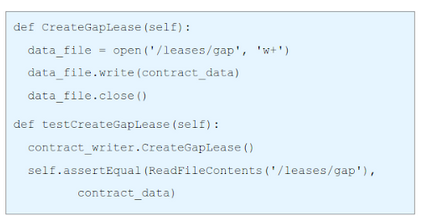
\includegraphics[width=1\textwidth]{esempioFlaky}
	\caption{\emph{Esempio flaky test}}
	\label{fig:mesh1}
\end{figure}

Il metodo “\emph{CreateGapLease}” apre il file “\emph{/leases/gap}” ed esegue la scrittura del contenuto della variabile “\emph{contract\_data}” al suo interno ed infine chiude il file.
Il test case “\emph{testCreateGapLease}” invoca la funzione “\emph{CreateGapLease}” e successivamente controlla che il contenuto del file “\emph{/leases/gap}” sia effettivamente
uguale al contenuto della variabile “\emph{contract\_data}”.
Ma cosa avviene nel momento in cui il file “\emph{/leases/gap}” esiste già e contiene già dati al suo interno? In questo caso il test genererà un fail. In questo caso il flaky
è dovuto semplicemente ad un errato controllo della precondizione del test, ma in generale errori di questo tipo possono capitare nei casi più disparati (es. in ambito di concorrenza, network etc.).
Una prima strategia di fix può essere quella di verificare l’effettiva esistenza del file “\emph{/leases/gap}” (eliminandolo in caso affermativo).
La figura 1.2 mostra il codice del metodo “testCreateGapLease” dopo la modifica.
\begin{figure}[h]
	\centering
	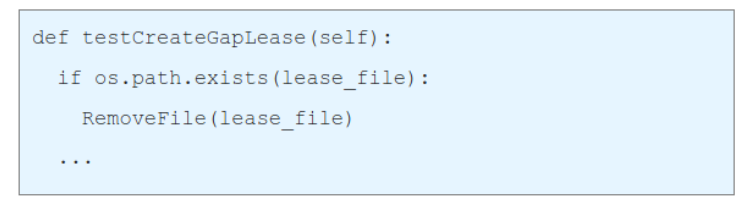
\includegraphics[width=1\textwidth]{figura1.2}
	\caption{\emph{Snippet di codice modificato}}
	\label{fig:mesh1}
\end{figure}

Tuttavia, neanche questa modifica è sufficiente per garantire la corretta esecuzione del caso di test in quanto, se “\emph{/leases/gap}” ha un path di tipo NFS e può essere scritto da un altro test, il metodo “\emph{testCreateGapLease}” può ancora fallire improvvisamente. La soluzione in questo caso consiste nell’effettuare alcune piccole modifiche al codice del metodo “\emph{CreateGapLease}” per rendere unica la
risorsa di cui ha bisogno.

La figura 1.3 mostra il codice del metodo “\emph{CreateGapLease}” dopo aver effettuato le opportune modifiche.
\newpage
\begin{figure}[h!]
	\centering
	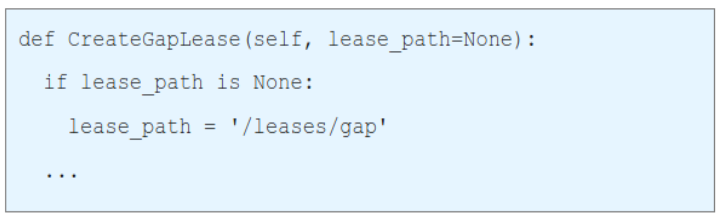
\includegraphics[width=1\textwidth]{figura1.3}
	\caption{\emph{Codice modificato}}
	\label{fig:mesh1}
\end{figure}

La chiamata al metodo “CreateGapLease” verrà effettuata nello stesso modo illustrato precedentemente, ma il test potrà passargli un path differente. Tale strategia impedirà fallimenti ad intermittenza del test case.

La figura 1.4 mostra il codice del metodo nella sua versione finale[6].
\begin{figure}[h!]
	\centering
	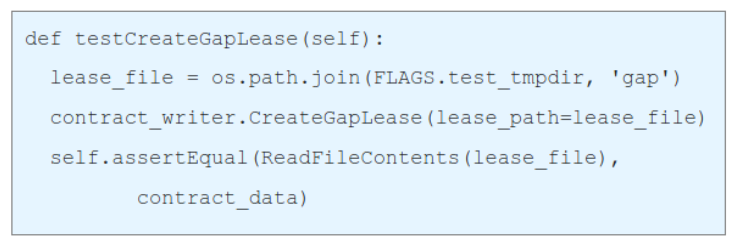
\includegraphics[width=1\textwidth]{figura1.4}
	\caption{\emph{Versione finale del codice}}
	\label{fig:mesh1}
\end{figure}